\subsection{$k$-Nearest Neighbours}
\label{sec:knn}
%\knn{} is a well known method in supervised learning, it is a 
%non-parametric method and a type of instance-based learning, or lazy 
%learning .\\

The overall \knn{} concept is simple: store the whole training set in 
the memory space, calculate the distance between the given test point 
to all training points, and apply the majority voting system to 
determine which class the test data sample belongs to.
Therefore, one of the advantages of using \knn{} is that it is 
intuitive and simple. Moreover, \knn{} algorithm has no training 
phase. 
%Third, it can easily be applied to multiclass classification 
%problem, we only need to modify the the voting system step. 
However, there are some shortcomes when applying \knn{}. As we 
mentioned above, \knn{} stores all training data in the memory space, 
therefore, the method will become slower as the training data 
increase, see Figure~\ref{fig:knncomp}.

Based on our knowledge and some implementation experiments, we came 
up with a modified \knn{} approach. 
First, we input the extracted ECG signal's features data into the 
algorithm, then it stores the training set. Second we input the 
testing data into the algorithm, and perform distance calculation 
between every points and save it. In order to increase the 
computation efficiency, we adjust the distance calculation step to 
have a more efficient way of selecting nearest neighbour without 
calculating every feature's distance between every data points. In 
order to decrease the sensitivity to outliers, we let the voting 
weight be the reciprocal of the function of Euclidean distance so the 
neighbour points near the testing point influence more. This 
technique puts greater emphasis on the reference samples that are 
closer to the test sample. 
So, the decision is less affected by training samples which are 
unstable in the feature space in comparison with other 
samples, and also filter out the outliers and noise. Finally we use 
a standard binary classification 0-1 loss to determine the overall 
accuracy and confusion matrix of the model, see Table~\ref{tbl:res}.

We analysed the training and test errors with respect to the number 
of neighbours (X-axis), see Figure~\ref{fig:knnerror}. Test error has 
the smallest value of $0.0563$ when $k=3$.

\paragraph{Implementation.}
ADD HERE

\begin{figure}
	\centering
	\begin{subfigure}{.5\textwidth}
		\centering
		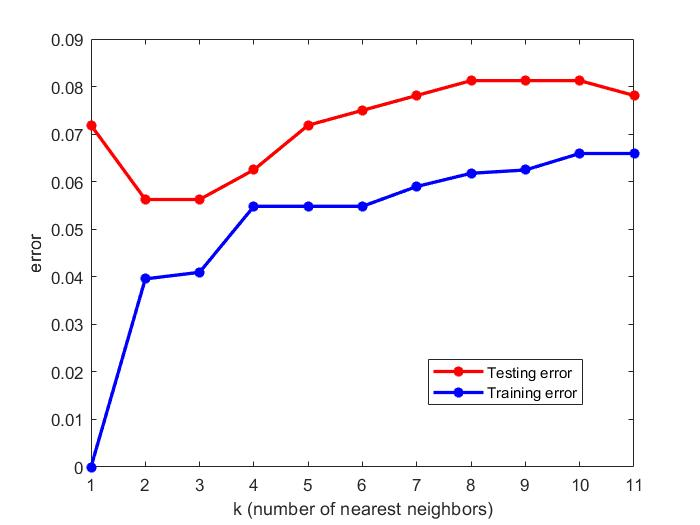
\includegraphics[width=.9\linewidth]{figures/knnerror.jpg}
		\caption{Error Plot}
		\label{fig:knnerror}
	\end{subfigure}%
	\begin{subfigure}{.5\textwidth}
		\centering
		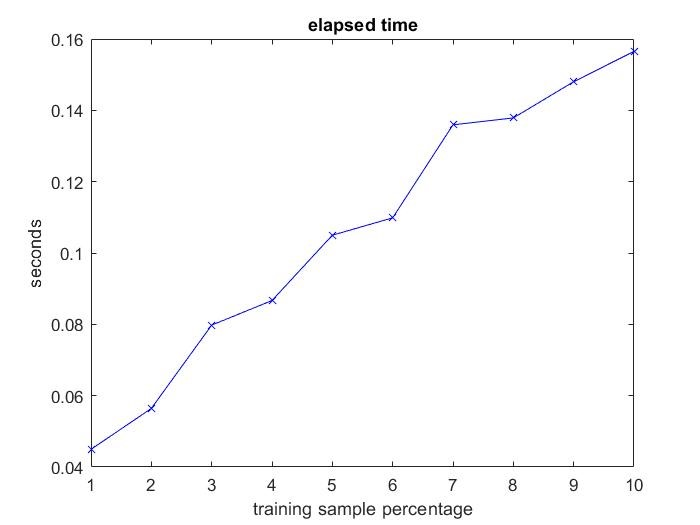
\includegraphics[width=.9\linewidth]{figures/knncomp.jpg}
		\caption{Computation Time}
		\label{fig:knncomp}
	\end{subfigure}
	\caption{\knn{} performance: training/test errors (left) and 
	computation time (right).}
	\label{fig:knn}
\end{figure}

%\begin{figure}[t]
%	\centering
%	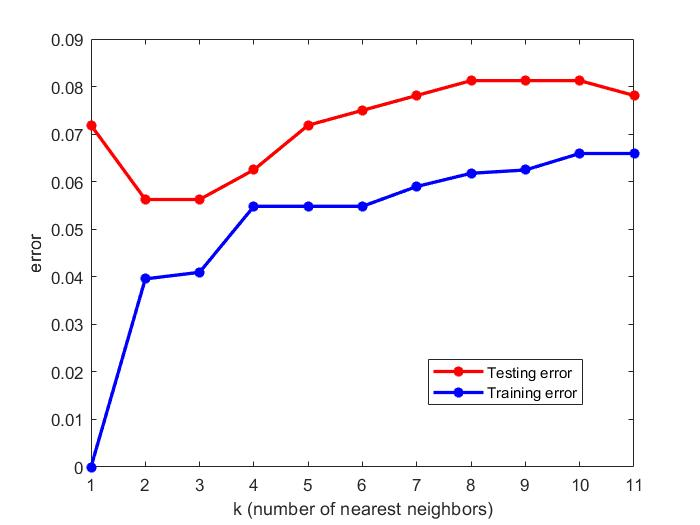
\includegraphics[width=0.6\textwidth]{figures/knnerror.jpg}
%	\caption{Error Plot}
%	\label{fig:knnerror}
%\end{figure}

%\begin{figure}[t]
%	\centering
%	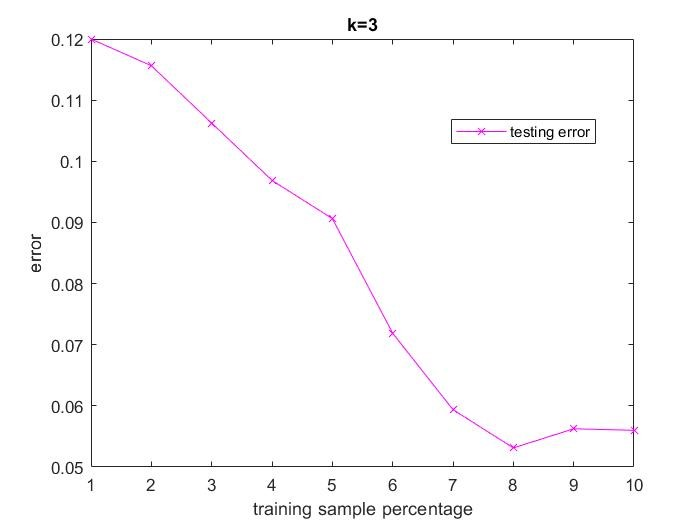
\includegraphics[width=0.6\textwidth]{figures/knntest.jpg}
%	\caption{Test Error}
%	\label{fig:knntest}
%\end{figure}

%\begin{figure}[t]
%	\centering
%	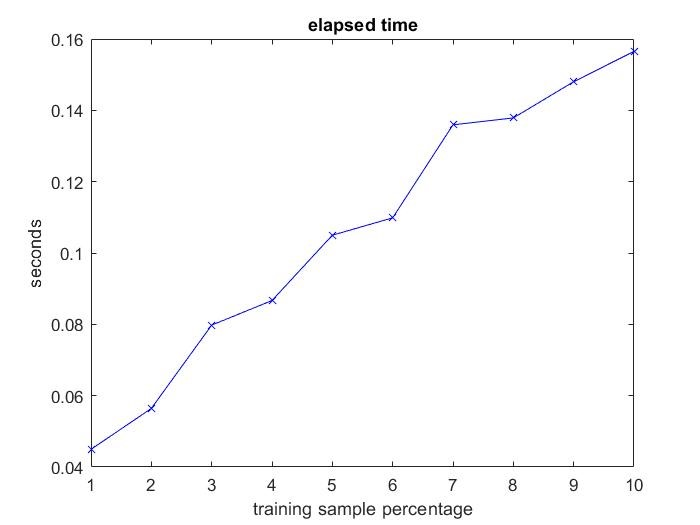
\includegraphics[width=0.6\textwidth]{figures/knncomp.jpg}
%	\caption{Computation Time}
%	\label{fig:knncomp}
%\end{figure}




%Figure~\ref{fig:knntest} shows that the test error decreases as the 
%training set becomes larger.









